% 第 1 章 §1.6–§1.7（印刷页 31–37）
\section{圈群的二聚体与可积系统}

本节的目标是陈述我们的主要结果：GK 可积系统的类与圈群 $\widehat{PGL}(N)$ 的 Poisson 子流形上自然定义的可积系统的类（§1.4.3）重合。

文献 [11] 证明了：若二部图 $\Gamma$ 是极小的，则作用映射 $I_\Gamma:B^2(\Sigma)\to\mathcal{M}$ 可积。换言之，所谓可积是指：归一化面配分函数
\[
S^f_\Gamma(\lambda,\boldsymbol{x})=\sum_i\mathcal{H}_i(\boldsymbol{x})\langle\boldsymbol{i},\boldsymbol{\lambda}\rangle
\]
的系数集合 $\{\mathcal{H}_i\}$ 彼此 Poisson 交换；并且，当略去归一化配分函数的角系数后，它们构成一个极大的、函数独立的运动积分交换族。

容易相信，这一构造给出的运动积分个数是极大的。为简单起见，设 Thurston 图的所有曲线都没有自交点。此时三重点的个数、从而白面的个数等于 $2S$，其中 $S$ 是 Newton 多边形 $\Delta$ 的面积（这可通过对 Newton 多边形取适当的三角剖分，并利用两条定向边的向量积等于 Thurston 图上相应曲线的相交指数来证明）。因此相空间的维数等于 $2S-1$。非平凡哈密顿量的个数等于属于 $\Delta$ 的整点的个数 $N$。Casimir 函数（Casimir function）的个数等于 $B-3$，其中 $B$ 是 $\Delta$ 的边界点的个数。于是运动积分的最大个数为 $(2S-1-(B-3))/2=S-B/2+1=N$，这是依 Pick 定理得到的。

此外，[11] 还证明了：

\begin{enumerate}[label=(\roman*),leftmargin=3em]
\item 若 $\boldsymbol{i}$ 是 Newton 多边形 $\Delta$ 的边界的一个角，则 $\mathcal{H}_i=c_i(\boldsymbol{x})$ 是 Casimir 函数（$\{x_i\}$ 中的单项式），即对 $B^2(\Sigma)$ 上的任意函数 $f=f(\boldsymbol{x})$ 都有 $\{\mathcal{H}_i,f\}=0$；
\item 两个极小图 $\Gamma_1$ 与 $\Gamma_2$ 能经由蛛形变换（见 §1.7.1）互相得到，当且仅当相应的多边形 $\Delta_1$ 与 $\Delta_2$ 能经由平移或 $\mathrm{SL}(2,\Z)$ 作用互相映射；这样的图称为等价的；
\item 对应于同一多边形的两个可积系统经由簇变换同构。
\end{enumerate}

因此，GK 可积系统由 Newton 多边形 $\Delta$ 列举，而其相空间上的坐标系由环面 $\Sigma$ 上的二部图 $\Gamma$ 列举。§1.4.3 中构造的 $\widehat{PGL}(N)$ 的 Poisson 子流形上的可积系统，由余扩张双外尔群（coextended double Weyl group）中循环不可约的元素 $u\in(\tilde W\times\tilde W)^{\sharp}$ 列举，而其相空间上的坐标由这些元素分解为生成元的约化词 $u=s_{i_1}\cdots s_{i_l}\Lambda^k$ 列举。我们需要在这两组数据之间建立对应。

首先用 Thurston 图把这两组组合数据都编码。确实，给定约化分解 $u=s_{i_1}\cdots s_{i_l}\Lambda^k$，我们可以在柱面上画出相应的 Thurston 图；再把该柱面的左右两边粘合起来，便得到环面上的图。相应的 Newton 多边形是 $H_1(\Sigma,\R)$ 中一个在平移下唯一的凸多边形，其各边是 Thurston 图上曲线的类。另一方面，Thurston 图与二部图 $\Gamma$ 一一对应，见附录 1.12。

现在，对任意 Newton 多边形 $\Delta$，都存在 $(\tilde W\times\tilde W)^{\sharp}$ 的生成元中的一个约化词 $s_{i_1}\cdots s_{i_l}\Lambda^k$，使得其粘合后的 Thurston 图的曲线对应于 $\Delta$ 的各边。在平面 $H_1(\Sigma,\R)$ 中选一个坐标系，使多边形的任何边都不竖直。于是多边形的每条边给出环面 $H_1(\Sigma,\R)/H_1(\Sigma,\Z)$ 上的一个圈。我们可以用切向量处处不竖直、且横截交点数最少的曲线来代表所有这些圈。用一条竖直线把环面剪开，就得到柱面上的一族曲线；这些曲线的条数，记为 $N$，将是多边形宽度的两倍（一半曲线向左，一半向右）。略去向左的曲线，就得到绕线图，以及与之对应的、生成元 $\{s_i\mid i\ge0\}$ 中的词，再乘以 $\Lambda^k$。幂 $k$ 由多边形最左与最右顶点的高度差给出。同样，略去向右的曲线，得到生成元 $\{\bar s_{\bar i}\mid \bar i\le0\}$ 中的一个词，再乘以同一个 $k$ 对应的 $\Lambda^k$。把这两个词以任意方式洗牌，再把结果乘以 $\Lambda^k$，就得到 $(\tilde W\times\tilde W)^{\sharp}$ 的生成元中的一个词，使得相应的 Thurston 图具有所要求的 Newton 多边形 $\Delta$。

对任意给定的约化词 $u\in(\tilde W\times\tilde W)^{\sharp}$，参数化胞腔 $G^u/\operatorname{Ad}H$ 的变量集合与 Thurston 图的白面集合（从而与环面 $\Sigma$ 上相应二部图 $\Gamma$ 的面集合）之间存在自然双射。确实，一方面，给定 $u$ 的一个约化分解，参数化变量的胞腔与生成元 $s_i$ 一一对应，而生成元对应于 Thurston 图的三重点。另一方面，在选定了竖直方向、且曲线切向量处处不竖直的环面上的 Thurston 图中，每个白面都有其最左交点，因此白面也由三重点列举。

\begin{theorem}\label{thm:1.6.1}
设 $u=s_{i_1}\cdots s_{i_l}\Lambda^k$ 是群 $\widehat{PGL}(N)$ 的余扩张双外尔群中的一个词，令 $S_u(\lambda,\mu;\boldsymbol{x})=\det(\mathcal{A}_u(\lambda,\boldsymbol{x})-\mu)$ 为在对应于给定分解的簇坐标 $\boldsymbol{x}$ 下参数化双 Bruhat 胞腔 $G^u/\operatorname{Ad}H$ 的矩阵的特征多项式。则该函数在相差一个归一化的意义下，等于由对应于词 $s_{i_1}\cdots s_{i_l}\Lambda^k$ 的 Thurston 图构造出的环面上的二部图的二聚体面配分函数。
\end{theorem}

本定理的证明大部分已经完成。给定既对应于词 $u=s_{i_1}\cdots s_{i_l}\Lambda^k$、同时又对应于图 $\Gamma$ 的 Thurston 图，可以用竖直的圆周把它剪成 $l$ 个初等块，每块内部恰有一个三重点。注意，每一块都对应于图 1.7 与图 1.8 中所示的某个图。只需比较二部图中绕面与绕之字形路径的单值性（计算配分函数 $S_u(\lambda,\mu,\boldsymbol{x})$ 时用到它们），并验证它们与按计算二聚体配分函数的规则所规定的绕面与绕之字形路径的单值性一致。

\section{变异与离散流}

\subsection{二部图的等价}

如 [11] 所示，在某些图变换下，面配分函数保持不变，至多差一个面变量 $\boldsymbol{x}$ 的簇变换（变异与投影的复合）。其中一个变换（图 1.9A）只是把与一个二价顶点相接的两条边缩掉，并保持各面上的变量不变。第二个变换即所谓的蛛形变换，见图 1.9C。此时面上的变量在菱形中央经变异而改变，其交换矩阵 $\varepsilon^{ij}$ 对应于 Poisson 括号 (1.35)。第三个变换从具有相同顶点的两条边中消去一条（图 1.9B）。该变换使变量个数减少一个，是变异与投影的复合。每个图都可约化为一个图，称为\emph{极小的}，其中变量个数不能再减少。

特别地，若这样一串变换保持图不变、却改变变量（从而给出相应簇代数簇的非平凡映射类群元素），则相应的映射保持 Poisson 结构与运动积分，因而与可积流交换。

\setcounter{figure}{8}
\begin{figure}[htbp]
\centering
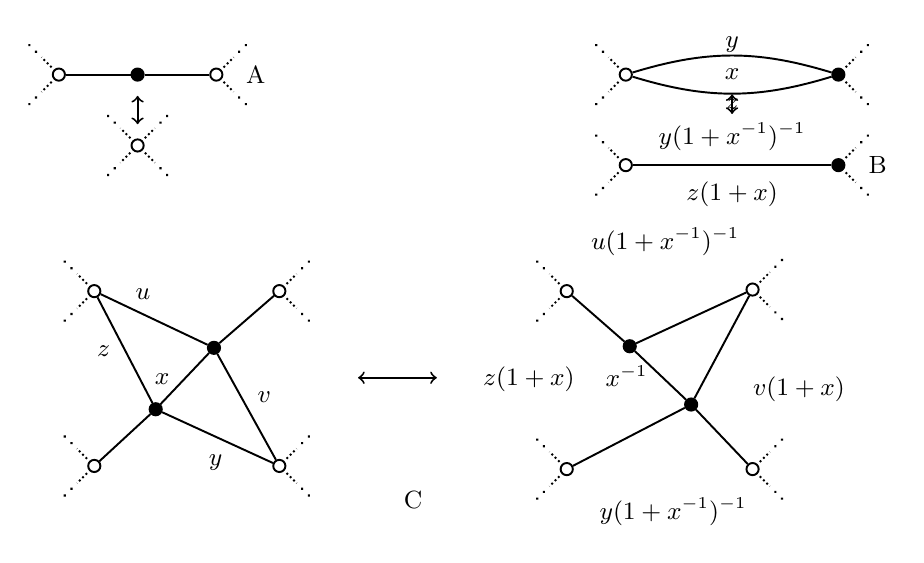
\begin{tikzpicture}[x=1cm,y=1cm,line width=0.7pt,font=\small]
\tikzset{
  vw/.style={circle,draw,minimum size=4.4pt,inner sep=0pt,fill=white},
  vb/.style={circle,draw,minimum size=4.4pt,inner sep=0pt,fill=black},
  cont/.pic={\draw[densely dotted] (0.13,0)--(0.31,0);
             \fill (0.41,0) circle (0.55pt);
             \fill (0.53,0) circle (0.55pt);}
}
% ---------- 面板 A：消去二价顶点 ----------
\node[vw] (a1) at (0.55,5.45) {};
\node[vb] (a2) at (1.55,5.45) {};
\node[vw] (a3) at (2.55,5.45) {};
\draw (a1)--(a2)--(a3);
\pic[rotate=135] at (a1) {cont};
\pic[rotate=225] at (a1) {cont};
\pic[rotate=45]  at (a3) {cont};
\pic[rotate=315] at (a3) {cont};
\draw[<->] (1.55,5.18)--(1.55,4.82);
\node[vw] (a4) at (1.55,4.55) {};
\pic[rotate=45]  at (a4) {cont};
\pic[rotate=135] at (a4) {cont};
\pic[rotate=225] at (a4) {cont};
\pic[rotate=315] at (a4) {cont};
\node at (3.05,5.45) {A};
% ---------- 面板 B：消去重边 ----------
\node[vw] (b1) at (7.75,5.45) {};
\node[vb] (b2) at (10.45,5.45) {};
\draw (b1) to[bend left=17] (b2);
\draw (b1) to[bend right=17] (b2);
\node at (9.10,5.83) {$y$};
\node at (9.10,5.45) {$x$};
\node at (9.10,5.08) {$z$};
\pic[rotate=135] at (b1) {cont};
\pic[rotate=225] at (b1) {cont};
\pic[rotate=45]  at (b2) {cont};
\pic[rotate=315] at (b2) {cont};
\draw[<->] (9.10,5.20)--(9.10,4.95);
\node[vw] (b3) at (7.75,4.30) {};
\node[vb] (b4) at (10.45,4.30) {};
\draw (b3)--(b4);
\node[anchor=south] at (9.10,4.36) {$y(1+x^{-1})^{-1}$};
\node[anchor=north] at (9.10,4.22) {$z(1+x)$};
\pic[rotate=135] at (b3) {cont};
\pic[rotate=225] at (b3) {cont};
\pic[rotate=45]  at (b4) {cont};
\pic[rotate=315] at (b4) {cont};
\node at (10.95,4.30) {B};
% ---------- 面板 C 左：蛛形变换之前 ----------
\node[vw] (c1) at (1.00,2.70) {};   % 左上
\node[vw] (c2) at (3.35,2.70) {};   % 右上
\node[vw] (c3) at (1.00,0.48) {};   % 左下
\node[vw] (c4) at (3.35,0.48) {};   % 右下
\node[vb] (c5) at (2.52,1.98) {};   % 上黑
\node[vb] (c6) at (1.78,1.20) {};   % 下黑
\draw (c1)--(c5); \draw (c5)--(c2);
\draw (c1)--(c6); \draw (c6)--(c3);
\draw (c5)--(c6); \draw (c6)--(c4);
\draw (c5)--(c4);
\foreach \p in {c1,c3} {\pic[rotate=135] at (\p) {cont}; \pic[rotate=225] at (\p) {cont};}
\foreach \p in {c2,c4} {\pic[rotate=45]  at (\p) {cont}; \pic[rotate=315] at (\p) {cont};}
\node at (1.62,2.66) {$u$};
\node at (1.12,1.94) {$z$};
\node at (1.86,1.58) {$x$};
\node at (2.54,0.52) {$y$};
\node at (3.16,1.36) {$v$};
% ---------- 面板 C 中：横向箭头 ----------
\draw[<->] (4.35,1.60)--(5.35,1.60);
% ---------- 面板 C 右：蛛形变换之后 ----------
\node[vw] (d1) at (7.00,2.70) {};   % 左上
\node[vw] (d2) at (9.36,2.72) {};   % 右上
\node[vw] (d3) at (7.00,0.44) {};   % 左下
\node[vw] (d4) at (9.36,0.44) {};   % 右下
\node[vb] (d5) at (7.80,2.00) {};   % 上黑
\node[vb] (d6) at (8.58,1.26) {};   % 下黑
\draw (d1)--(d5); \draw (d5)--(d2);
\draw (d5)--(d6); \draw (d2)--(d6);
\draw (d6)--(d3); \draw (d6)--(d4);
\foreach \p in {d1,d3} {\pic[rotate=135] at (\p) {cont}; \pic[rotate=225] at (\p) {cont};}
\foreach \p in {d2,d4} {\pic[rotate=45]  at (\p) {cont}; \pic[rotate=315] at (\p) {cont};}
\node[anchor=south] at (8.25,3.02) {$u(1+x^{-1})^{-1}$};
\node at (7.76,1.62) {$x^{-1}$};
\node at (6.52,1.58) {$z(1+x)$};
\node[anchor=north] at (8.35,0.20) {$y(1+x^{-1})^{-1}$};
\node at (9.95,1.45) {$v(1+x)$};
\node at (5.05,0.05) {C};
\end{tikzpicture}
\caption{A：消去一个二价顶点；B：消去一条重边；C：蛛形变换。}
\label{fig:1.9}
\end{figure}

\subsection{离散流 $\tau$}

回忆变换 $\tau$ 定义在 $G/\operatorname{Ad}H$ 上，也定义在 Poisson 子流形 $G^u/\operatorname{Ad}H$ 上，为 $\tau(g_-g_+)=g_+g_-$，其中 $g_-$ 与 $g_+$ 分别属于下 Borel 子群与上 Borel 子群。对群 $\widehat{PGL}(N)$，可用 $\tau(g_-g_+)=g_+\Lambda^kg_-\Lambda^{-k}$ 推广这一变换。这个变换显然保持由生成函数 $\det(g\Lambda^k-\mu)$ 给出的可积系统的哈密顿量。

任意 $u\in(\tilde W\times\tilde W)^{\sharp}$ 都容许分解 $u=s_{i_1}\cdots s_{i_l}\Lambda^k$，其中 $i_1,\dots,i_p$ 为正、$i_{p+1},\dots,i_l$ 为负（例如可以从任一分解出发，利用负生成元与正生成元彼此交换，把前者移到右边、把后者移到左边）。这样的分解可以如下变形：
\[
\begin{aligned}
u&=s_{i_1}\cdots s_{i_l}\Lambda^k=s_{i_1}\cdots s_{i_p}s_{i_{p+1}}\cdots s_{i_l}\Lambda^k
\sim s_{i_{p+1}}\cdots s_{i_l}\Lambda^ks_{i_1}\cdots s_{i_p}\\
&=s_{i_{p+1}}\cdots s_{i_l}s_{i_1+k}\cdots s_{i_p+k}\Lambda^k
=s_{i_1+k}\cdots s_{i_p+k}s_{i_{p+1}}\cdots s_{i_l}\Lambda^k=u',
\end{aligned}
\]
其中 $\sim$ 表示生成元的循环移位；第二个与第四个等号由负生成元与正生成元的交换性得到，第三个等号由关系 $\Lambda s_i=s_{i+1}\Lambda$ 得到。这串等式与循环移位诱导出从 $G^u/\operatorname{Ad}H$ 到 $G^{u'}/\operatorname{Ad}H$ 的态射。特别地，显然当 $k=0$ 时 $u=u'$，我们得到 $G^u/\operatorname{Ad}H$ 的保持运动积分的自同构。这个自同构正是变换 $\tau$。若 $k\ne0$，则把同一变换重复 $N/\gcd(k,N)$ 次，给出一个自同构，我们也把它记作 $\tau$。

\subsection{一般离散流}

取一个 Newton 多边形 $\Delta$，考虑相应的、由 Thurston 变换相联系的一列 Thurston 图，其中第一个图与最后一个图重合。这样的序列定义了相应簇代数簇 $\mathcal{X}_\Delta$（见附录 1.9）的一个自同构（可能是平凡的），它保持 §1.6 的可积系统。这样的自同构构成我们的可积系统的离散自同构群 $\mathcal{G}_\Delta$。尽管迄今我们还没有这个群的完整描述，但我们仍将给出一个离散阿贝尔群 $\mathcal{G}'_\Delta$ 的组合构造（其中 $\Delta$ 是 Newton 多边形），并定义相应可积系统的离散自同构群到 $\mathcal{G}'_\Delta$ 的同态。我们猜想这个同态实际上是同构。

设 $\Z^{|V_\Delta|}$ 为 Newton 多边形 $\Delta$ 的顶点集 $V_\Delta$ 上整值函数的群。设 $A$ 是 $V_\Delta$ 上可延拓为整系数仿射函数的函数构成的子群，即形如 $aX+bY+c$ 的函数，其中 $a,b,c\in\Z$，而 $(X,Y)$ 是 $H_1(\Sigma)=\Z^2$ 上的坐标。我们的群定义为商 $\mathcal{G}'_\Delta=\Z^{|V_\Delta|}/A$。显然这个群的秩等于 $|V_\Delta|-3$，但一般它有非平凡的挠。\begin{annote}原文此处作 “were $a,b,c\in\Z$”，其中 were 当为 where 之误，译文按 where 的本意处理。[来源：上下文推断]\end{annote}

现在描述同态 $\mathcal{G}_\Delta\to\mathcal{G}'_\Delta$。取一列由 Thurston 变换相联系、代表 $\mathcal{G}_\Delta$ 中元素的 Thurston 图。任何这样的序列都可以用单参数的曲线族来插值，使得除有限多个参数值外所有交点都是三重的，而对每个其余的参数值允许一个对应于这些变换的四重交点。由于第一个图与最后一个图重合，可以设参数属于单位圆 $S^1$。考虑乘积 $\Sigma\times S^1$。Thurston 图的每条曲线在这个乘积中描出一个曲面。若 $\Sigma$ 是环面 $T^2$，则 $\Sigma\times S^1$ 是三维环面 $T^3$，而每个圈定义同调群 $H_2(T^3,\Z)=\Z^3$ 中的一个元素。于是我们得到 $H_2(T^3,\Z)$ 中的一列点 $\delta_1,\dots,\delta_K$，Newton 多边形 $\Delta$ 的每条边对应一个。

确切地说，设下标按 $\Delta$ 各边的逆时针顺序、从最右顶点开始编号。这样一族圈的圈之和 $\sum_r\delta_r$ 在同调中为零。确实，圈之补集的连通分支从 Thurston 图继承灰色与白色的染色。因此圈之和是（比如说）灰色分支之并的边界。

在 $H_1(T^3,\Z)$ 中取同调基 $e^1,e^2,e^3$，其中 $e^1,e^2$ 是 $H_1(T^2,\Z)$ 的基。这个基诱导出 $H_2(T^3,\Z)$ 的基 $e^{kl}=e^k\wedge e^l$（$k<l$）。记类 $\delta_i$ 在此基下的坐标为 $(a^i_{12},a^i_{23},a^i_{13})$。由于 $\sum_i a^i_{12}=0$，存在 $\Delta$ 的顶点上的一族数 $\{f^i\}$（差一个常数确定），使得对 $i\in\Z/K\Z$ 有 $a^i_{12}=f^{i+1}-f^i$。这族数定义了 $\mathcal{G}'_\Delta$ 的元素。

注意，若 Thurston 图的一条曲线代表圈 $Xe^1+Ye^2$，并且它平移 $ae^1+be^2$，则 $T^3$ 上相应的圈由
\[
(Xe^1+Ye^2)\wedge(ae^1+be^2+e^3)=(bX-aY)e^{12}+Xe^{13}+Ye^{23}
\]
给出。考虑所有曲线的平移 $ae^1+be^2$ 都相同的情形。若 $a$、$b$ 是整数，则相应的自同构是平凡的，而 $\mathcal{G}'_\Delta$ 中相应的元素也平凡，因为它由仿射函数 $bX-aY$ 给出。这个论证表明同态的构造是合理的。另一方面，若 $X$ 与 $Y$ 是有理数，但所有坐标 $a^{kl}_i$ 都是整数，则 $\mathcal{G}'_\Delta$ 中相应的元素是挠元素。\begin{annote}原文此处作 $a^{kl}_i$，与本段前面所用的 $a^i_{kl}$ 记号不一致，译文照排。[来源：上下文推断]\end{annote}

现在考虑 §1.7.2 中定义的自同构 $\tau$。用 Thurston 图的语言，这对应于把定向为从右到左的那一族圈整体平移，而保持其余圈不动。为了回到原来的圈构形，需要把该族按向量 $(Ne^1+ke^2)/\gcd(k,N)$ 平移。向量 $Ne^1+ke^2$ 正是连接 Newton 多边形 $\Delta$ 最左与最右顶点的向量。这个向量把 Newton 多边形切成两部分。相应的函数 $f_i$ 可以取为：在上半部分为零；在下半部分为在该向量上消失、并在整数点上取整数值的极小非零线性函数。

正如 A. B. Goncharov 向我们指出的，群 $\mathcal{G}_\Delta$ 还有另一种解释。即：Newton 多边形定义了一个环面曲面 $M_\Delta$，以及其上由谱曲线代表的一个同调类（见 [8, §3.4]）。多边形的边对应于无穷远除子的各分支。$M_\Delta$ 上的 Picard 群限制到一般谱曲线的 Picard 群。群 $\mathcal{G}_\Delta$ 是次数为零的线丛的原像。换言之，群 $\mathcal{G}_\Delta$ 是谱曲线上那些可延拓为 $M_\Delta$ 上的线丛的线丛构成的群。我们猜想：离散流经由相应的线丛作乘法而作用在谱曲线的 Jacobian 上。
